\documentclass[9pt,twocolumn,twoside,]{pnas-new}

% Use the lineno option to display guide line numbers if required.
% Note that the use of elements such as single-column equations
% may affect the guide line number alignment.


\usepackage[T1]{fontenc}
\usepackage[utf8]{inputenc}

% tightlist command for lists without linebreak
\providecommand{\tightlist}{%
  \setlength{\itemsep}{0pt}\setlength{\parskip}{0pt}}




\templatetype{pnasresearcharticle}  % Choose template

\title{Template for preparing your research report submission to PNAS
using RMarkdown}

\author[a,1]{Gabrielle Bibeau}
\author[a]{Laura Glaude}
\author[a]{Emmanuelle Langlois}
\author[a]{Cloé Tanguay}

  \affil[a]{Université de Sherbrooke, Département de Biologie, 2500
Boulevard de l'Université, Sherbrooke, Québec, Canada}


% Please give the surname of the lead author for the running footer
\leadauthor{Anonymous}

% Please add here a significance statement to explain the relevance of your work
\significancestatement{Authors must submit a 120-word maximum statement
about the significance of their research paper written at a level
understandable to an undergraduate educated scientist outside their
field of speciality. The primary goal of the Significance Statement is
to explain the relevance of the work in broad context to a broad
readership. The Significance Statement appears in the paper itself and
is required for all research papers.}


\authorcontributions{Please provide details of author contributions
here.}



\correspondingauthor{\textsuperscript{1} À qui la correspondance devrait
être addressée. Courriel:
\href{mailto:bibg1101@usherbrooke.ca}{\nolinkurl{bibg1101@usherbrooke.ca}}}

% Keywords are not mandatory, but authors are strongly encouraged to provide them. If provided, please include two to five keywords, separated by the pipe symbol, e.g:
 \keywords{  Benthos |  Biodiversité  } 

\begin{abstract}
Please provide an abstract of no more than 250 words in a single
paragraph. Abstracts should explain to the general reader the major
contributions of the article. References in the abstract must be cited
in full within the abstract itself and cited in the text.
\end{abstract}

\dates{This manuscript was compiled on \today}
\doi{\url{www.pnas.org/cgi/doi/10.1073/pnas.XXXXXXXXXX}}

\begin{document}

% Optional adjustment to line up main text (after abstract) of first page with line numbers, when using both lineno and twocolumn options.
% You should only change this length when you've finalised the article contents.
\verticaladjustment{-2pt}



\maketitle
\thispagestyle{firststyle}
\ifthenelse{\boolean{shortarticle}}{\ifthenelse{\boolean{singlecolumn}}{\abscontentformatted}{\abscontent}}{}

% If your first paragraph (i.e. with the \dropcap) contains a list environment (quote, quotation, theorem, definition, enumerate, itemize...), the line after the list may have some extra indentation. If this is the case, add \parshape=0 to the end of the list environment.

\acknow{Merci à Victor Cameron et Benjamin Mercier sans qui ce projet
n'aurait été possible.}

This PNAS journal template is provided to help you write your work in
the correct journal format. Instructions for use are provided below.

Note: please start your introduction without including the word
``Introduction'' as a section heading (except for math articles in the
Physical Sciences section); this heading is implied in the first
paragraphs.

\hypertarget{guide-to-using-this-template}{%
\section*{Guide to using this
template}\label{guide-to-using-this-template}}
\addcontentsline{toc}{section}{Guide to using this template}

Please note that whilst this template provides a preview of the typeset
manuscript for submission, to help in this preparation, it will not
necessarily be the final publication layout. For more detailed
information please see the
\href{http://www.pnas.org/site/authors/format.xhtml}{PNAS Information
for Authors}.

Emma (introduction, pas de titre pcq c'est ce qui est recommandé dans le
template de l'article et je trouvais que ça ferait professionnel)

\hypertarget{muxe9thodes}{%
\subsubsection*{Méthodes}\label{muxe9thodes}}
\addcontentsline{toc}{subsubsection}{Méthodes}

Le jeu de données utilisé contient une partie des inventaires du benthos
faits par le ministère de l'Environnement, de la Lutte contre les
Changements Climatiques, de la Faune et des Parcs (MELCCFP) dans le
cadre du suivi de la qualité de l'eau des rivières du Québec. Ces
données, extraites du site Biodiversité Québec, recensent les espèces de
macroinvertébrés benthiques vivant dans les rivières du Québec.
L'échantillonnage a été réalisé en suivant le protocole
d'échantillonnage des macroinvertébrés benthiques d'eau douce du Québec.

Avant l'analyse des données, celles-ci sont passées à travers plusieurs
étapes de manipulations. Premièrement, les données, extraites sous forme
d'une multitude de fichiers .csv, ont été manipulées pour être jointes
en une seule matrice. Deuxièmement, la matrice a été nettoyée, notamment
en assignant une classe pertinentes aux valeurs de la matrice (ex: les
dates en format `Date' et non en format `Character'), en enlevant les
colonnes importunes (ne contenant que des NAs ou étant des doublons) et
en remplaçant les données problématiques par des NAs (valeurs de -99
pour des variables ayant des valeurs réalistiquement positives).
Troisièmement, des numéros d'identification (IDs) ont été assignés pour
toutes les combinaisons de dates, de sites et d'heures. Finalement, une
base de données .db a été créer pour entreposer deux tables : une tables
contenant des informations reliées aux IDs de sites et une table
contenant des informations sur les abondances des taxons de benthos
identifiés.

Différentes analyses ont été performées sur les données pour répondre
aux questions posées par ce rapport. D'abord, des régressions linéaires
simples (p=0.05) de la richesse spécifique ont été produites en fonction
des variables suivantes : la largeur de la rivière, la profoncdeur de la
rivière, la vitesse du courant et la température de l'eau. Ensuite, un
diagramme à moustache validé par un test de t avec un interval de
confiance de 0.95 a été réalisé pour la richesse spécifique en fonction
de la transparence de l'eau. Puis, une vérification d'intéractions pour
toutes les combinaisons possibles de variables abiotiques a été conduite
avec des régressions linéaires simples (p=0.05). La majorité des
variables (toutes sauf la température de l'eau) n'ont pas une
distribution normale. Toutefois, suite à des tests de régressions
linéaires généralisées avec différentes familles (par exemple la
poisson), nous en sommes venues à la conclusion que les erreurs avaient
une plus belle distribution (normale) lorsque nous utilisions la
régression linéaire simple. Finalement, une ordination de type PCoA
(Principal Coordinates Analysis) de la composition en abondance des
communatés benthiques a été produite seulement avec les échantillons
pris plus d'une fois (à des moments différents) sur un même site. Aucun
tests statistiques n'a été réalisé pour confirmer la significativité des
observations permises par l'outil de visualisation qu'est l'ordination.

\hypertarget{ruxe9sultats}{%
\subsubsection*{Résultats}\label{ruxe9sultats}}
\addcontentsline{toc}{subsubsection}{Résultats}

Nous avons d'abord testé l'effet des différentes variables abiotiques
(largeur de la rivière, profondeur de la rivière, transparence de l'eau,
température de l'eau et vitesse du courant) sur la richesse spécifique
des échantillons analysés. Les régressions linéaires à la figure
\ref{fig:regression_richesse} nous permettent d'observer un effet
significatif pour la variable de la température, mais pas pour les
autres.

\begin{figure}
\centering
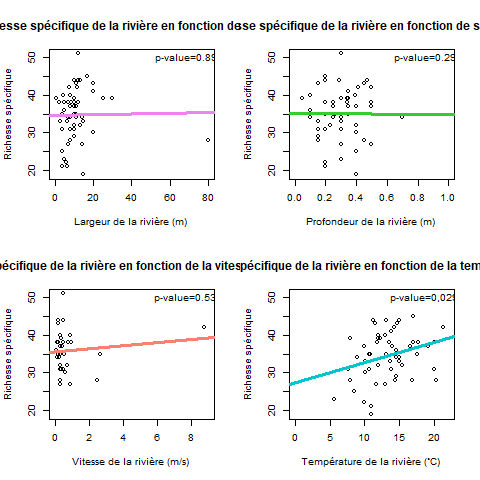
\includegraphics{regression_richesse.png}
\caption{Régressions linéaires de la richesse en fonction de (A) la
largeur de la rivière, (B) la profoncdeur de la rivière, (C) la vitesse
du courant et (D) la température de l'eau.
\label{fig:regression_richesse}}
\end{figure}

L'effet de la transparence a été visualié en diagramme à moustache
plutôt qu'en régression linéaire. Il s'avère que cette variable
n'affecte pas non plus significativement la richesse spécifique des
communautés de benthos.

\begin{figure}
\centering
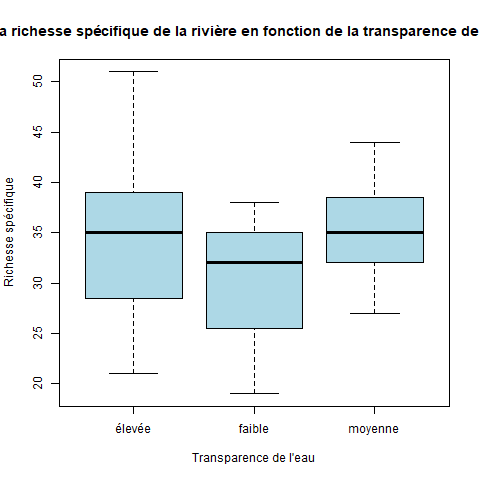
\includegraphics{boxplot_richesse.png}
\caption{Diagramme à moustache de la richesse spécifique des
échantillons de benthos en fonction de la transparence de l'eau lors de
l'échantillonnage. \label{fig:boxplot_richesse}}
\end{figure}

Ensuite, nous avons vérifié s'il y avait des interactions entre les
variables. Selon le tableau de la figure \ref{fig:tableau_interaction},
il n'y a aucune interaction significative entre les variables abiotiques
en ce qui concerne la richesse spécifique des échantillons.

\begin{figure}
\centering
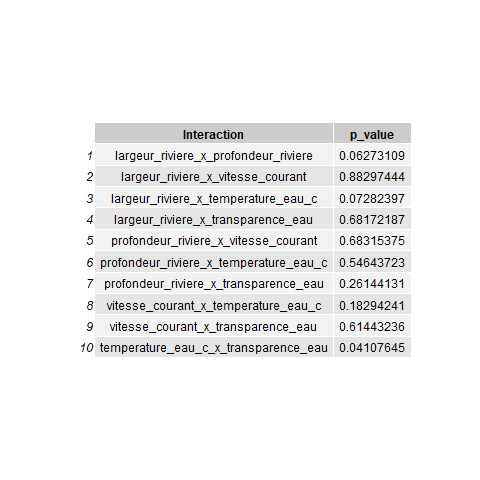
\includegraphics{tableau_interaction.png}
\caption{Tableau de la significativité des interactions entre les
variables affectant la richesse spécifique des échantillons dans des
régressions linéaires. \label{fig:tableau_interaction}}
\end{figure}

Finalement, la diversité beta a été observé à l'aide d'une ordination
PCoA. À l'oeil, sur la figure \ref{fig:ordination_sites}, certains sites
semblent avoir des commuanutés de benthos similaires entre les
différentes périodes d'échantillonnages, alors que d'autres sont plutôt
variées. Entre-eux, les sites sont parfois très proches en terme de
composition même s'ils sont différents géographiquement, d'autres fois
complètement différents.

\begin{figure}
\centering
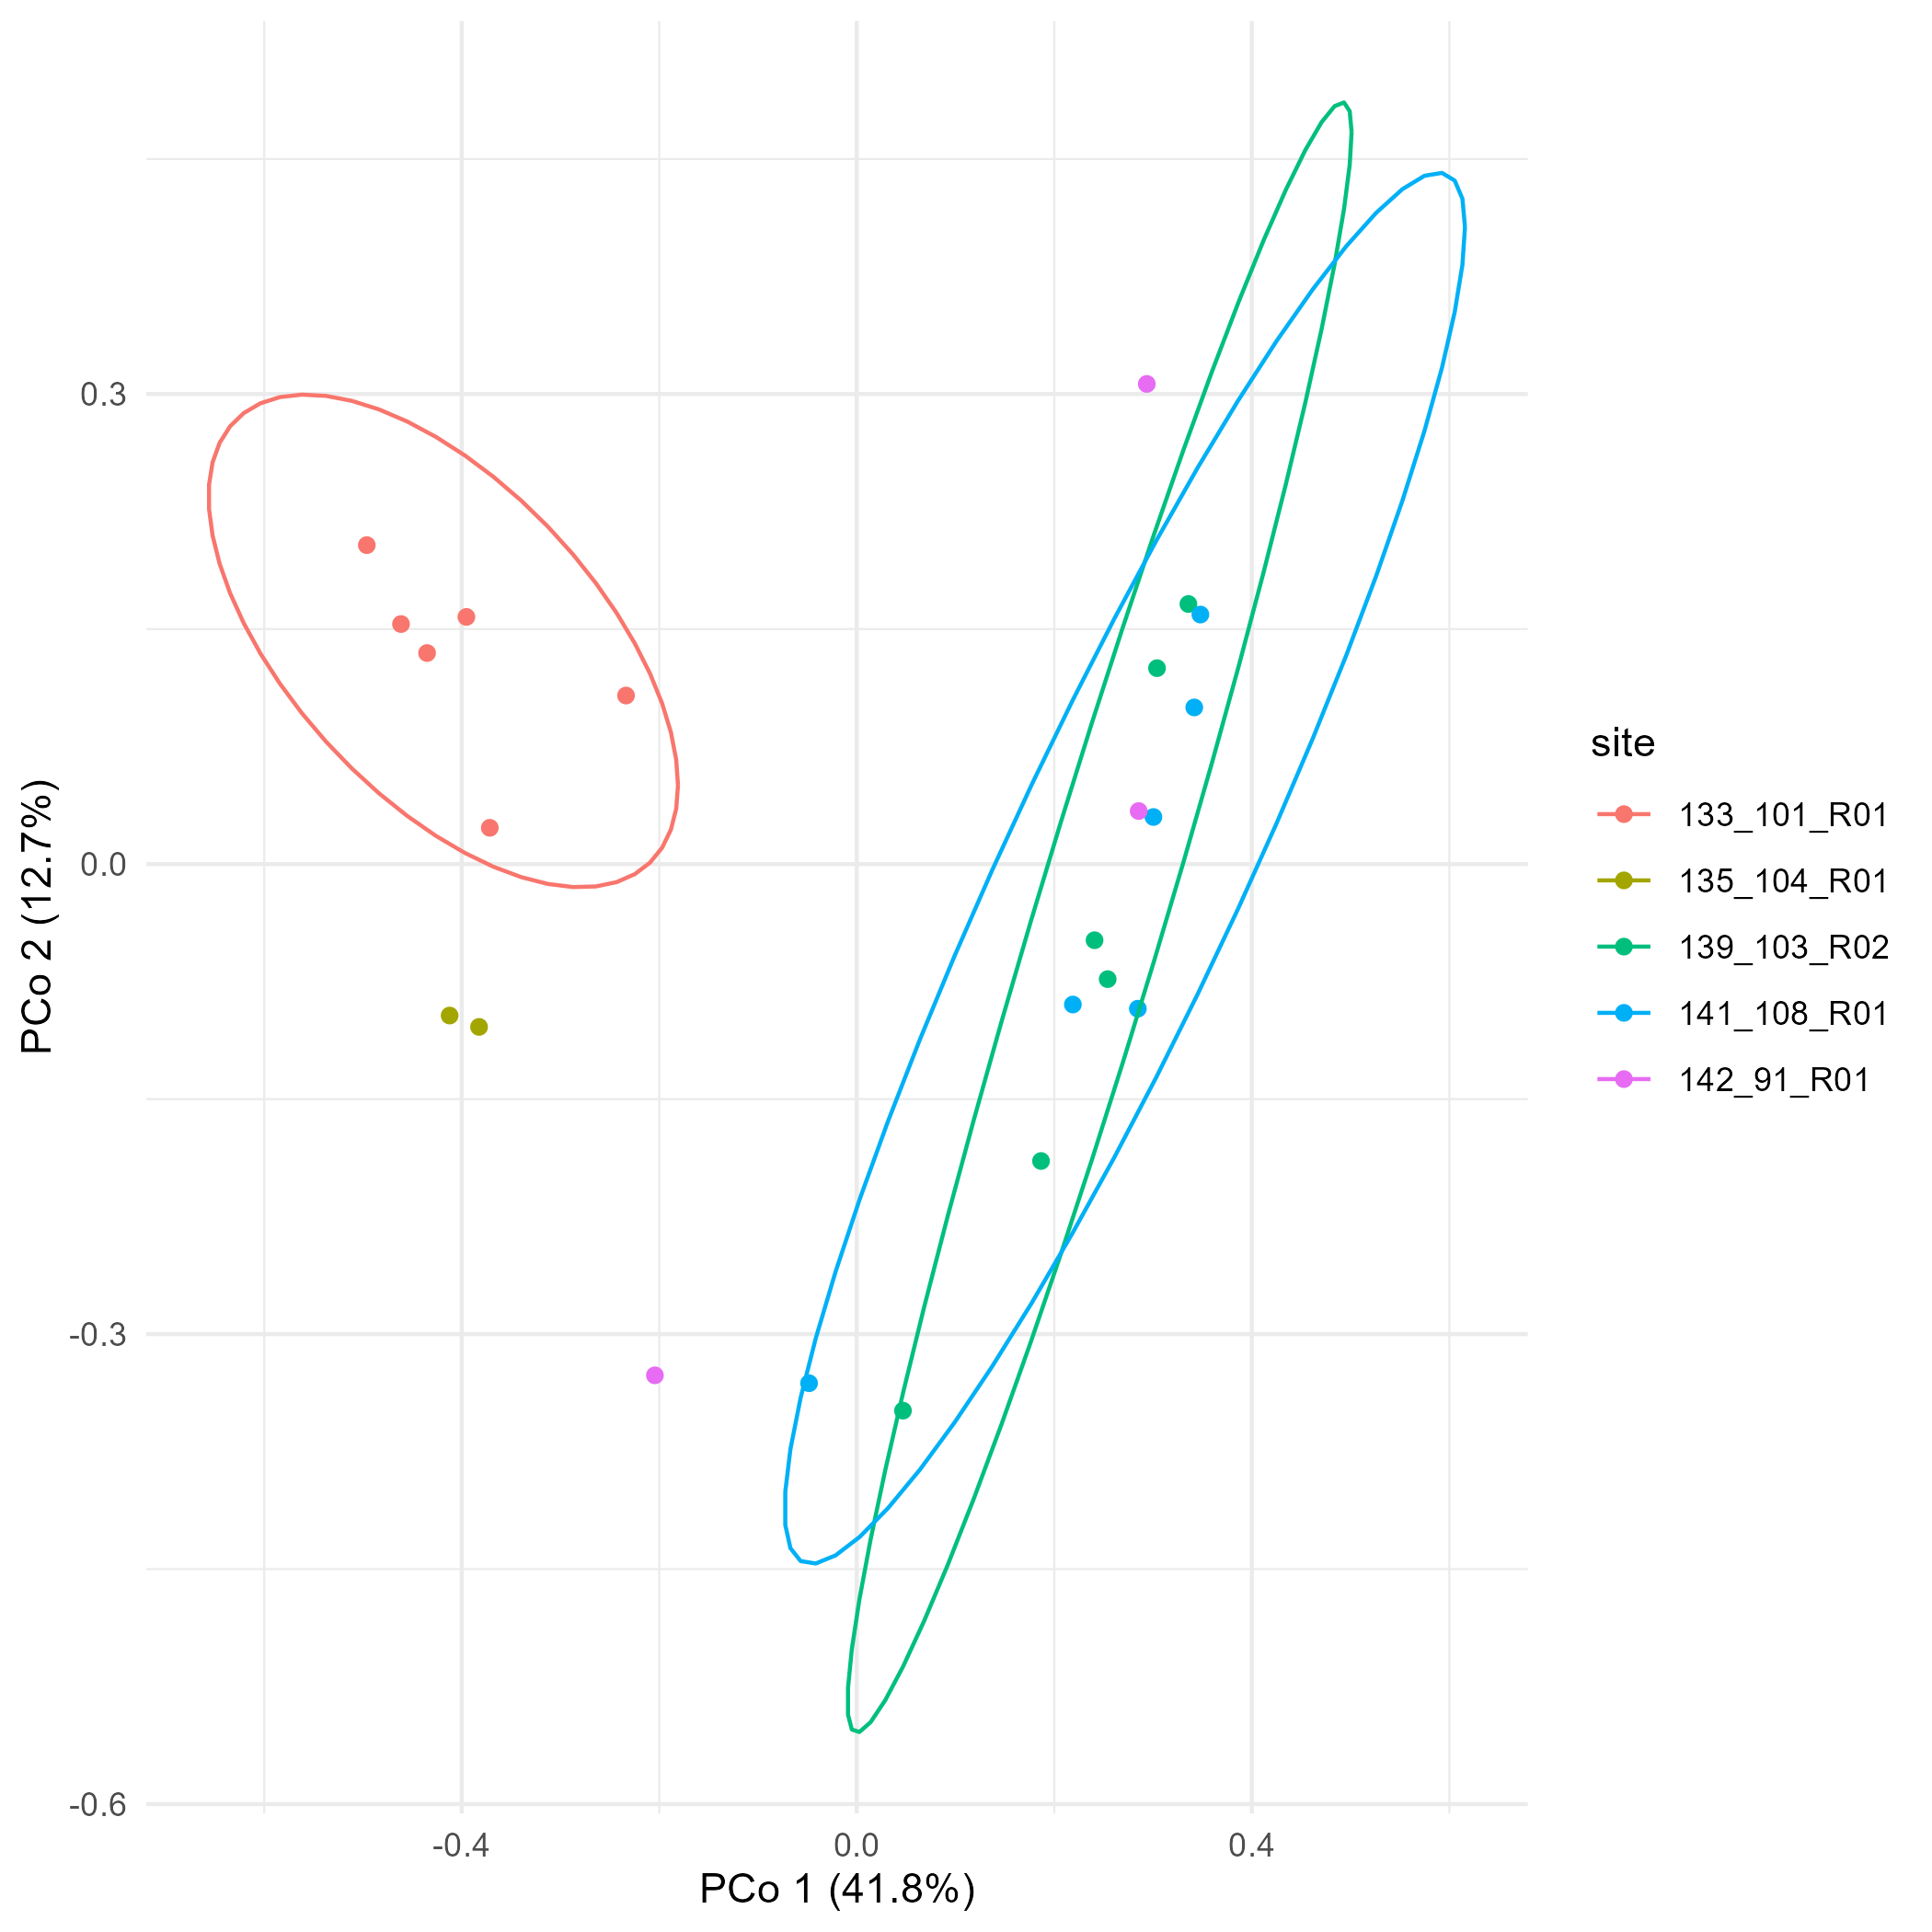
\includegraphics{ordination_sites.png}
\caption{PCoA des communautés de benthos échantillonnées par
Biodiversité Québec en fonction du site. \label{fig:ordination_sites}}
\end{figure}

\hypertarget{discussion}{%
\subsubsection*{Discussion}\label{discussion}}
\addcontentsline{toc}{subsubsection}{Discussion}

Les résultats ne donnent que très peu d'information quant aux variables
expliquant la diversité du benthos. Mise à part la température, aucun
facteur d'habitat ne donne de résultat significatif. La littérature
mentionne clairement l'impact de la température sur les communautés
benthiques, mais l'effet des autres variables reste incertain (Jowett,
2003; Godson et al., 2022). Une relation entre la vélocité, largeur et
profondeur des rivières a déjà été démontrée, mais elle ne semble pas
s'appliquer aux petits cours d'eau (Jowett, 2003). De plus, la vélocité
devrait être mesurée au niveau du substrat, l'espace occupé par le
benthos, plutôt que dans la colonne d'eau, ce qui pourrait expliquer que
les résultats obtenus ne sont pas significatifs (Jowett, 2003). De plus,
plusieurs variables faisant parties des plus importantes, telles que les
caractéristiques du substrat, n'ont pas été testées dû à l'absence de
données (Jowett, 2003; Godson et al., 2022). D'autres caractéristiques
de l'habitat peuvent affecter la structure des populations d'invertébrés
benthiques lorsqu'elles sont mises en relation avec les caractéristiques
des sédiments (Jowett, 2003; Godson et al., 2022). Il serait donc
pertinent d'ajouter ces mesures au protocole de caractérisation du
milieu dans les futures études. Aussi, les tests n'ont été effectués que
sur un échantillon de données de benthos disponibles. Augmenter la
quantité de données pourrait également augmenter les chances d'obtenir
des résultats significatifs.

\showmatmethods
\showacknow
\pnasbreak



% Bibliography
% \bibliography{pnas-sample}

\end{document}
